\documentclass{article}
\usepackage{graphicx}
% ascunde blocurile de referinta cu `hidelinks`
\usepackage[hidelinks]{hyperref}

\begin{document}

% \quad - adauga un tab de 4 spatii. pus la primele paragrafe din fiecare sectiune pentru % a pastra consistenta vizuala 

%%%%%%%%%%%%%%%%%%%%%%%%%%%%% pag 1 %%%%%%%%%%%%%%%%%%%%%%%%%%%%%%%%%%%%%
\begin{figure}
    
\includegraphics{images/unitbv.png}
\end{figure}

\title{ETICA ÎN DOMENIUL INTELIGENȚEI ARTIFICIALE}
\author{Lucian Florin Rus\\ \\Facultatea de Matematică și Informatică\\Informatică - ID, anul I}

\date{04 Ianuarie 2026}
\maketitle

\tableofcontents
% incheie pagina mai repede din considerente estetice
    \newpage

%%%%%%%%%%%%%%%%%%%%%%%%%%%%% pag 2 %%%%%%%%%%%%%%%%%%%%%%%%%%%%%%%%%%%%%
\section{Abstract}
\quad Prezenta lucrare își propune sintetizarea atât a informațiilor legate de implementarea \textit{Inteligenței Artificiale} (notată și \textbf{IA}), \textbf{într-o manieră cât mai simplă}, cât și enumerarea și explicarea celor 4 principii care stau la baza eticii în domeniul acesteia. Detaliile de implementare prezentate în această lucrare sunt considerate esențiale, acestea formând contextul necesar înțelegerii principiilor anterior menționate.

\section{Introducere}

\quad Inteligența artificială reprezintă capacitatea unui sistem computațional de a imita activități și funcții care, de regulă, sunt asociate cu inteligența umană. Exemple de astfel de funcții și activități includ învățarea, percepția, rezolvarea problemelor și luarea de decizii bazate pe factori determinați și analizați anterior.

\subsection{Rețeaua neuronală}
\quad Deși există mai multe modalități de a implementa IA, metoda cea mai des utilizată, exemplificată, de altfel, și în această lucrare, este de a folosi o \textit{Rețea Neuronală} (notată și \textbf{RN}) \cite{g4g-nn}. O astfel de rețea se regăsește în imaginea alăturată.

\begin{figure}[h]
    \centering
    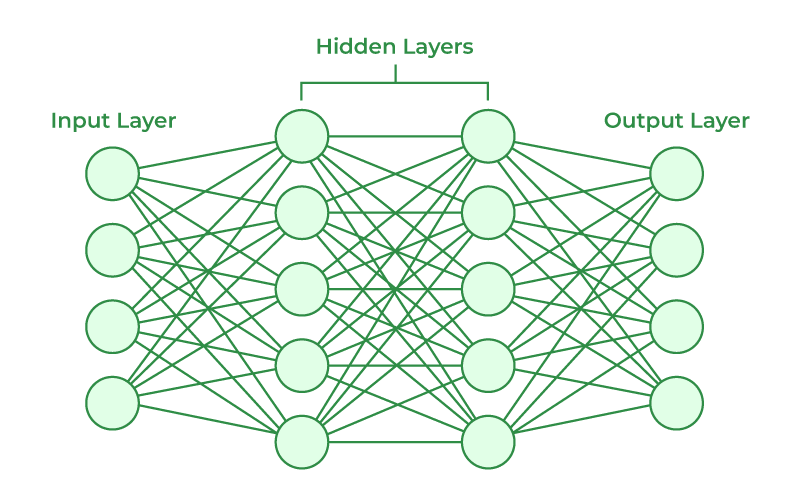
\includegraphics[width=\textwidth]{images/nn-architecture.png}
    \caption{Exemplu de rețea neuronală la scară mică}
    \label{fig:rn-ref}
\end{figure}

% incheie pagina mai repede din considerente estetice
\newpage
%%%%%%%%%%%%%%%%%%%%%%%%%%%%% pag 3 %%%%%%%%%%%%%%%%%%%%%%%%%%%%%%%%%%%%%
Folosind \ref{fig:rn-ref} că referință, se poate observa că o Rețea Neuronală este compusă, de regulă, din 3 nivele:

\begin{itemize}
    \item nivelul de intrare
    \item nivelul de procesare (ascuns)
    \item nivelul de ieșire
\end{itemize}

Fiecare dintre aceste nivele conține o serie de neuroni, numărul acestora fiind dat de complexitatea activității pe care Rețeaua Neuronală trebuie să o îndeplinească. Detalierea implementării \textit{Neuronului Artificial} se va face într-un capitol ulterior. Acești neuroni sunt conectați prin intermediul muchiilor, astfel rezultând într-un sistem în care un neuron aparțînător unui nivel oarecare este conectat la toți neuronii din fiecare dintre nivele învecinate. Pentru ca sistemul să funcționeze, este necesară "antrenarea" acestuia, acest proces constând în calibrarea tuturor neuronilor din nivelul de procesare in baza unui set de date care constituie nivelul de intrare și a unui set de date care constituie nivelul de ieșire. Astfel, rețeaua neuronală va repeta acest proces, numit și \textbf{backpropagation} ori de câte ori este nevoie până la atingerea unui grad ridicat de încredere că rezultatul este unul corect.

\subsection{Neuronul Artificial}

\begin{figure}[h]
    \centering
    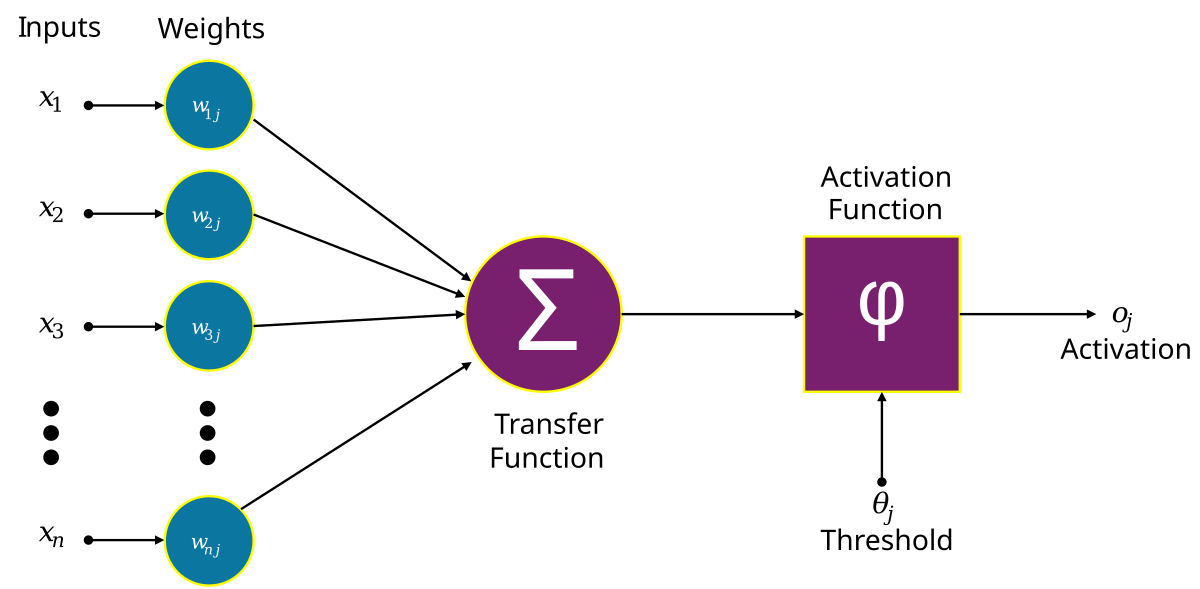
\includegraphics[width=\textwidth]{images/an-struct.png}
    \caption{Structura unui neuron artificial}
    \label{fig:an-ref}
\end{figure}

Neuronul artificial reprezintă unitatea de baza a unei Rețele Neuronale. În esență, neuronul este o entitate decizională foarte simplă a cărui scop este de a decide dacă datele de intrare sunt propagate la următorul nivel sau sunt întoarse pentru recalculare. Condiția care determina această decizie se numește \textbf{funcție de activare} \cite{g4g-af} și este referentiata în ecuația \ref{eq:1}.

%%%%%%%%%%%%%%%%%%%%%%%%%%%%% pag 4 %%%%%%%%%%%%%%%%%%%%%%%%%%%%%%%%%%%%%
\begin{equation}
    \centering
    \sigma(x) = \frac{1}{1 + e^{-x}}
    \label{eq:1}
\end{equation}

Datele de intrare (notate ca $x_i$ primite de neuron sunt adunate într-o suma ponderată, unde ponderea (notate ca $w_i$) reprezintă "importanța" aceastei informații. Rezultatul sumei este apoi trecut prin funcția de activare, similar cu ecuația \ref{eq:2}.

\begin{equation}
    \centering
    \sigma(w_1x_1 + w_2x_2 + w_3x_3+...+w_nx_n)
    \label{eq:2}
\end{equation}

\textbf{Bias}-ul unui neuron (notat ca \textit{b}) are rolul de a mitiga potențialele probleme cauzate de date de intrare nule și este adesea ales și adaptat de către dezvoltatorii rețelei neuronale în funcție de rezultatele antrenamentelor anterioare și este adunat sumei ponderate, similar cu ecuația \ref{eq:3}.

\begin{equation}
    \centering
    \sigma(w_1x_1 + w_2x_2 + w_3x_3+...+w_nx_n+b)
    \label{eq:3}
\end{equation}

O demonstrație vizuală a întregului proces în care un neuron este antrenat în cadrul unui sistem menit să recunoască numere scrise de mâna se poate găși si în video-ul \textbf{But what is a neural network?} \cite{3b1b}.

% incheie pagina mai repede din considerente estetice
\newpage

%%%%%%%%%%%%%%%%%%%%%%%%%%%%% pag 5 %%%%%%%%%%%%%%%%%%%%%%%%%%%%%%%%%%%%%
\section{Etica în domeniul IA}
\quad Etica în domeniul Inteligenței Artificiale are la baza 4 principii fundamentale. Apariția acestor principii, însă, nu a fost un eveniment singular ci o evoluție continuă care a avut loc concomitent cu evoluția tehnologiei propriu-zise, evoluție la care au contribuit nu doar cercetători ci și filosofi, scriitori și oameni de afaceri care au conștientizat potențialele riscuri. Aceste 4 principii sunt:
\begin{itemize}
    \item asigurarea transparenței
    \item asigurarea echității și a non-discriminării
    \item asigurarea confidențialitatea și securitatea
    \item asumarea responsabilității
\end{itemize}

În baza acestor principii, atât cercetătorii cât și dezvoltatorii de soluții și produse care se bazează pe IA se angajează să mitigheze potențialele riscuri prezentate de această tehnologie . La momentul scrierii acestei lucrări, din cauza lipsei unei baze legislative solide în mare parte din țările în care IA se folosește, principiile sunt respectate în mod voluntar, Uniunea Europeană, Canada, China și Brazilia fiind printre puținele jurisdicții în care IA este pusă sub semnul conformității. \cite{verifywise}.

\subsection{Transparența}
\quad Deciziile luate de un sistem care folosește IA trebuie să fie clare și să poată fi explicate și înțelese de către oameni, în special în situații în care este vorba despre subiecte care pot afecta viață oamenilor (de ex.: întrebări medicale, juridice, financiare etc.)

\subsection{Echitate și non-discriminare}
\quad Algoritmii care stau la baza unui model de IA trebuie să fie antrenați pe un set de date cât mai variat și divers pentru a evita posibilitatea apariției unui \textbf{bias}. Astfel, IA nu trebuie să perpetueze niciun fel de prejudecăți, deciziile luate bazându-se pe date factuale și obiective, complet agnostice de eventualele \textit{bias}-uri pe care utilizatorii le pot prezența.

\subsection{Confidențialitate și securitate}
\quad Sistemele care folosesc IA trebuie să respecte cu strictețe confidențialitatea și securitatea vieții private a utilizatorilor, evitând colectarea de date despre aceștia fără acordul lor explicit. Adesea, acest principiu constă în anonimizarea datelor, asigurarea cailor de comunicare și respectarea legislației din jurisdicția în care sistemul este folosit. 

%%%%%%%%%%%%%%%%%%%%%%%%%%%%% pag 6 %%%%%%%%%%%%%%%%%%%%%%%%%%%%%%%%%%%%%
\subsection{Responsabilitate}
\quad Trebuie să existe mecanisme clare de stabilire a răspunderii în eventualitatea în care un sistem care folosește IA greșește sau cauzează daune. 

\section{Abrevieri și explicații}
\subsection{Abrevieri}

Tabelul de mai jos conține o lista de abrevieri folosite in cadrul acestei lucrări. \newline


\begin{tabular}{ | c | l | } % { |c|l|c| } - pentru borduri complete
\hline % - linie deasupra
IA & inteligență artificială \\ 
\hline
RN & rețea neuronală  \\
\hline
\end{tabular}

\subsection{Explicatii}

Tabelul de mai jos conține o lista de termeni care pot necesita mai multe detalii, folosiți în cadrul acestei lucrări.\newline


\begin{tabular}{ | c | l | } % { |c|l|c| } - pentru borduri complete
\hline
bias & - avantajarea în mod conștient a cuiva în detrimentul altuia \\ % - fără newline de aici, \hline nu merge
\hline % - linie deasupra
\end{tabular}


% incheie pagina mai repede din considerente estetice
\newpage

%%%%%%%%%%%%%%%%%%%%%%%%%%%%% pag 7 %%%%%%%%%%%%%%%%%%%%%%%%%%%%%%%%%%%%%

\begin{thebibliography}{9}
\bibitem{g4g-nn}
\href{https://www.geeksforgeeks.org/machine-learning/neural-networks-a-beginners-guide/}{What is a Neural Network?}

\bibitem{g4g-af}
\href{https://www.geeksforgeeks.org/machine-learning/activation-functions-neural-networks/}{Activation functions in Neural Networks}

\bibitem{3b1b}
\href{https://www.youtube.com/watch?v=aircAruvnKk}{3Blue1Brown (2017), But what is a neural network?}

\bibitem{verifywise}
\href{https://verifywise.ai/lexicon/jurisdictional-compliance-in-ai}{Jurisdictional compliance in AI}

\end{thebibliography}

\end{document}


